\documentclass[14pt]{article}

\usepackage[margin=1in]{geometry}
\usepackage[utf8]{inputenc}
\usepackage{graphicx}

\title{Software Engineering project Phase 1\\Hospital Management System}
\author{Tareq Kirresh, Alaa Shuqair, Dua Abu Safiah, Ashjan Bakri}
\begin{document}
\begin{figure}[t!]
\centering
  
\includegraphics[width=7cm]{LOGO.png}
\end{figure}
\maketitle
\newpage
\tableofcontents 
\newpage 
\section{Introduction}
\subsection{State of the Customer}
The Customer is a Hospital, and currently, is completely dependant on a pen-and-paper process to perform all of its management. Our goal
is to transfer this process to an electronic one and streamline it, further adding features that allow the patient to be more 
directly involved in their treatment process. 
\subsection{Current Problems}
As stated above, the customer is still using a paper process for management. Due to the large number of patients and doctors, this 
has become very cumbersome on the customer for the following reasons:
\begin{enumerate}

	
	\item Breakdown in communication: Due to the fact that everything is being done by paper, sometimes the different departments
	do not get their message across clearly due to human errors in spelling or handwriting, leading to the need to repeat work.
	
	\item Theft: Due to the nature of the customer's buisness, no patient is turned away, and some are lying and claiming perscriptions
	and tests that were not written for them, costing the customer money, and due to the fact that the stock system is manual, the customer
	suspects that some things are taken out without permission. The customer would like to be able to control stocks better.
	
	\item Stocks: Due to the fact that there is no active change in stocks, the customer often finds themselves out of nescessary items.
	
	\item Protocol and Chain of command: The customer has said that due to the high amount of personal interaction and the slow speed of the 
	current system, Protocols are being breached often and the Chain of command is not being adhered to in order to provide care in a 
	timely fashion. 
	
	\item Storage issues: Due to the large amounts of records they have, the customer is running out of physical space to store 
	records of their operation. This will lead them to either rent an archive space or to destroy old records.
	
	\item Pollution: Since the customer still uses paper, this paper will eventually have to be destroyed, which is currently 
	through burning. The customer has stated that they would like to be more environmentaly-friendly and cut waste.
	
	
\end{enumerate}
\newpage
\section{Requirments}
\subsection{Functional Requirments}
\subsubsection{User Requirments}
\begin{enumerate}

\item The system shall allow patients to sign up an account.

\item The system shall have a log in for all users of all types. For hopital staff, there will also be a specialized page for 
them to log onto work.

	
\item The system shall allow the patient to ask for appointments, communicate with his doctor, see the doctor's notes and
perscriptions , and pay his bills via bank transfer or visa.

\item The system shall allow the receptionist  to register patiens, make appointments, and search for information about a patient.

\item The system shall allow the doctor to see patient details and stats,enter a diagnosis for a patient, give them perscriptions, nominate
them for surgery, request tests from the laboratory, reserve the operation theatre, and add special notes about the patient.

\item The system shall allow the nurse to see what the doctor's notes are for a patient,
ask the pharmacy for medicine, update patient status, and page for a patient's doctor.

\item The system shall allow the pharmacist to withdraw medicine(based on doctor requests or perscriptions), maintain stocks(count current
stocks and order new stock), view what standing perscriptions and past perscriptions the patient has, and produce stock reports.

\item The system shall allow the laboratory tech to see what tests were requested for a patient, enter the test results,
and maintain laboratory stocks.

\item The system shall connect to the current accounting system at the hospital, and the accounting system will be able to see
all relevant data to produce a bill and allow the patient to pay it as stated above. Patient billing data will also be produced based
on the accounting system

\item The system shall allow the admin to manage all accounts(create/delete/update), modify all data, see all reports,
view all bills, and see all stocks.
\end{enumerate}
\newpage
\subsubsection{System Requirments}
\begin{enumerate}
	\item \begin{enumerate}
			\item Upon opening the appropriate browser page, there will be 2 buttons, one will be sign up, the other will be log in.
			\item Upon opening the sign up page, the patient will be asked to enter their first name, last name, phone number,
			government ID number, email, and a password.
			\item Upon sucessfull sign up, the user will be transfered to the login page.
			\item doctors, pharmacists, lab techs, and nurses are signed up by a special page avaiable only to the admin and are assigned
			an account type.
			\end{enumerate}
	\item \begin{enumerate}
			\item Upon opening the appropriate browser page, there will be 2 buttons, one will be sign up, the other will be log in.
			\item Upon opening the log in page, the user will be asked to enter their email and paswords. Logins detected from 
			inside the hospital LAN that are from the @hospital.com domain will be redirected to a page appropriate to the account type
			assigned to them (eg, doctors are taken to their homepage, nurses to another, etc). Patients will be taken to a dash. Staff will 
			be taken to a page for them to log onto work. after they press log onto work,
			the time is sent to the HR system(that they currently use),then they are redirected to their main page.
		  \end{enumerate}
		  
	\item \begin{enumerate}
			\item The patient dash is a screen where the patient is given the most relevant information about them.
			\item The patient is shown any upcoming apointments, any outstanding perscriptions or bills, and any doctor orders.
			\item There will be a button that allows the patient to create a new appointment with a doctor
			\item There will be a button that allows the patient to start a chat with their doctor or call them via VOIP if they are 
			available, 
			\item There will be a payment screen for any outstanding bills, which is done through a visa or a bank account transfer. 
			\item Aditionally, there will be screens for a patient to view their billing history, diagnosis history, perscription history,
			and appointment history.
		  \end{enumerate}
		  
	\item \begin{enumerate}
			\item the receptionist main page has the buttons and menus for the receptionist to 
				\begin{enumerate}
					\item Create a new user for a patient.
					\item Search for an already registered patient.
					\item Look at a patient's data.
					\item Create an appointment for a patient. 
					\item message and call other hospital staff.
				\end{enumerate}
			\item sign out of work and log off.
		  \end{enumerate}
		  
		\item \begin{enumerate}
			\item the doctor main page has the buttons and menus for the doctor to 
				\begin{enumerate}
					\item See their schedule.
					\item Look at a patient's data.
					\item Place their notes about the patient.
					\item Create a new perscription for a patient.
					\item Request a test for a patient.
					\item Nominate a patient for surgery and reserve the operating theatre. 
					\item message and call other hospital staff.
				\end{enumerate}
			\item sign out of work and log off.
		  \end{enumerate}
		\item \begin{enumerate}
			\item the nurse main page has the buttons and menus for the nurse to 
				\begin{enumerate}
					\item Look at a patient's data.
					\item Read the doctor's notes about a patient.
					\item Request Medicine for a patient.
					\item Update the patient's status, in that, the time they were checked in, what ward they are in, what time
					they were given medicine, if they are deteriorating or doing fine, and if they have given them something other
					than what the doctor has ordered.
					\item Emergency page the doctor assigned to the patient(on their pager, not on the system).
					\item message and call other hospital staff.
				\end{enumerate}
			\item sign out of work and log off.
		  \end{enumerate}
	\item \begin{enumerate}
		\item the pharmacist main page has the buttons and menus for the pharmacist to 
				\begin{enumerate}
					\item Look at a patient's data.
					\item Read the doctor's notes about a patient.
					\item withdraw medicine for a patient from the stock based on their 
					perscription . The amount available in stock will go down acordingly. if the
					stock is at a critical level(less than 15 \% of normal stock), then the pharmacist will be notified.
					\item Place orders for new stock, and send them to purchascing department .
					\item Produce stock reports, which are a list of every medicine available by its brand name, current stock, and date. 
					Each entry in the list has a sublist of the time and amount of every withdrawl, along with which patient it was withdrawn
					for and which pharmacist withdrew it.
					\item message and call other hospital staff.
				\end{enumerate}
			\item sign out of work and log off.
		  \end{enumerate}
		  
		\item \begin{enumerate}
		\item the lab tech main page has the buttons and menus for the lab tech to 
				\begin{enumerate}
					\item Look at a patient's data.
					\item Read the doctor's notes about a patient.
					\item See what tests the doctor has ordered for a patient.
					\item Withdraw items used in tests(eg test tubes, litmus paper, etc), and be notified whenever the
					number is below a threshold(less than 15\% of the normal stock).
					\item Enter the results of the tests he has performed. Each test will have its own page depending on the test. 
					we are curently working together with the lab techs to create the form needed to be filled out for each test.
					\item Produce stock reports, which are a list of every perishable 
					item used in tests available by its brand name, current stock, and date. 
					Each entry in the list has a sublist of the time and amount of every withdrawl, along with which patient it
					was withdrawn for and which technitian withdrew it.
					\item Order stock and send it to the purchacing department.
					\item message and call other hospital staff.
				\end{enumerate}
			\item sign out of work and log off.
		  \end{enumerate}
		  
		 \item \begin{enumerate}
		\item The accounting system shall be connected to this system by means of the available API. 
		\item Patient billing data in this system is based on the data in the accounting system.
		\item This system allows a patient to pay via visa or bank transfer. 
		\item Note: Cash and cheque payments go through the present accounting system and not this one. 
		  \end{enumerate}
		  
		\item \begin{enumerate}
		\item The admin page has a button that takes the admin to the database management interface(eg PHPmyadmin).
		all modification of data will be done manually from there.
		\item The admin page has buttons that lead to a page where new staff are signed up and assigned an account type.
		\item The admin page has menus that allow the admin to see all reports in the hospital. 
		\item message and call other hospital staff.
		\item sign out of work and log off.
		  \end{enumerate}
		  
		
\end{enumerate}

\subsection{Non-Functional Requirments}
\begin{enumerate}
	\item The system shall be secured, With all paswords at least hashed and trafic being encrypted with at least https.
	\item The system shall guarantee patient-doctor confidentiality by ensuring that only authorized
	persons see specific data related to their work only.
	\item The system must not take more than 1 day of training to learn to use.
	\item The system must be responsive; No request shall take more than 2 seconds to be processed.
	\item The system must have an uptime of at least 99.9 \%.{}
	\item The system must implement the API's for visa and bank payments and the API's for the accounting and HR softwares.
	\item The system must have integrated VOIP and Pager capability. 
\end{enumerate}
\newpage
\section{Use Case Diagram}
\begin{figure}[h!]
\centering
  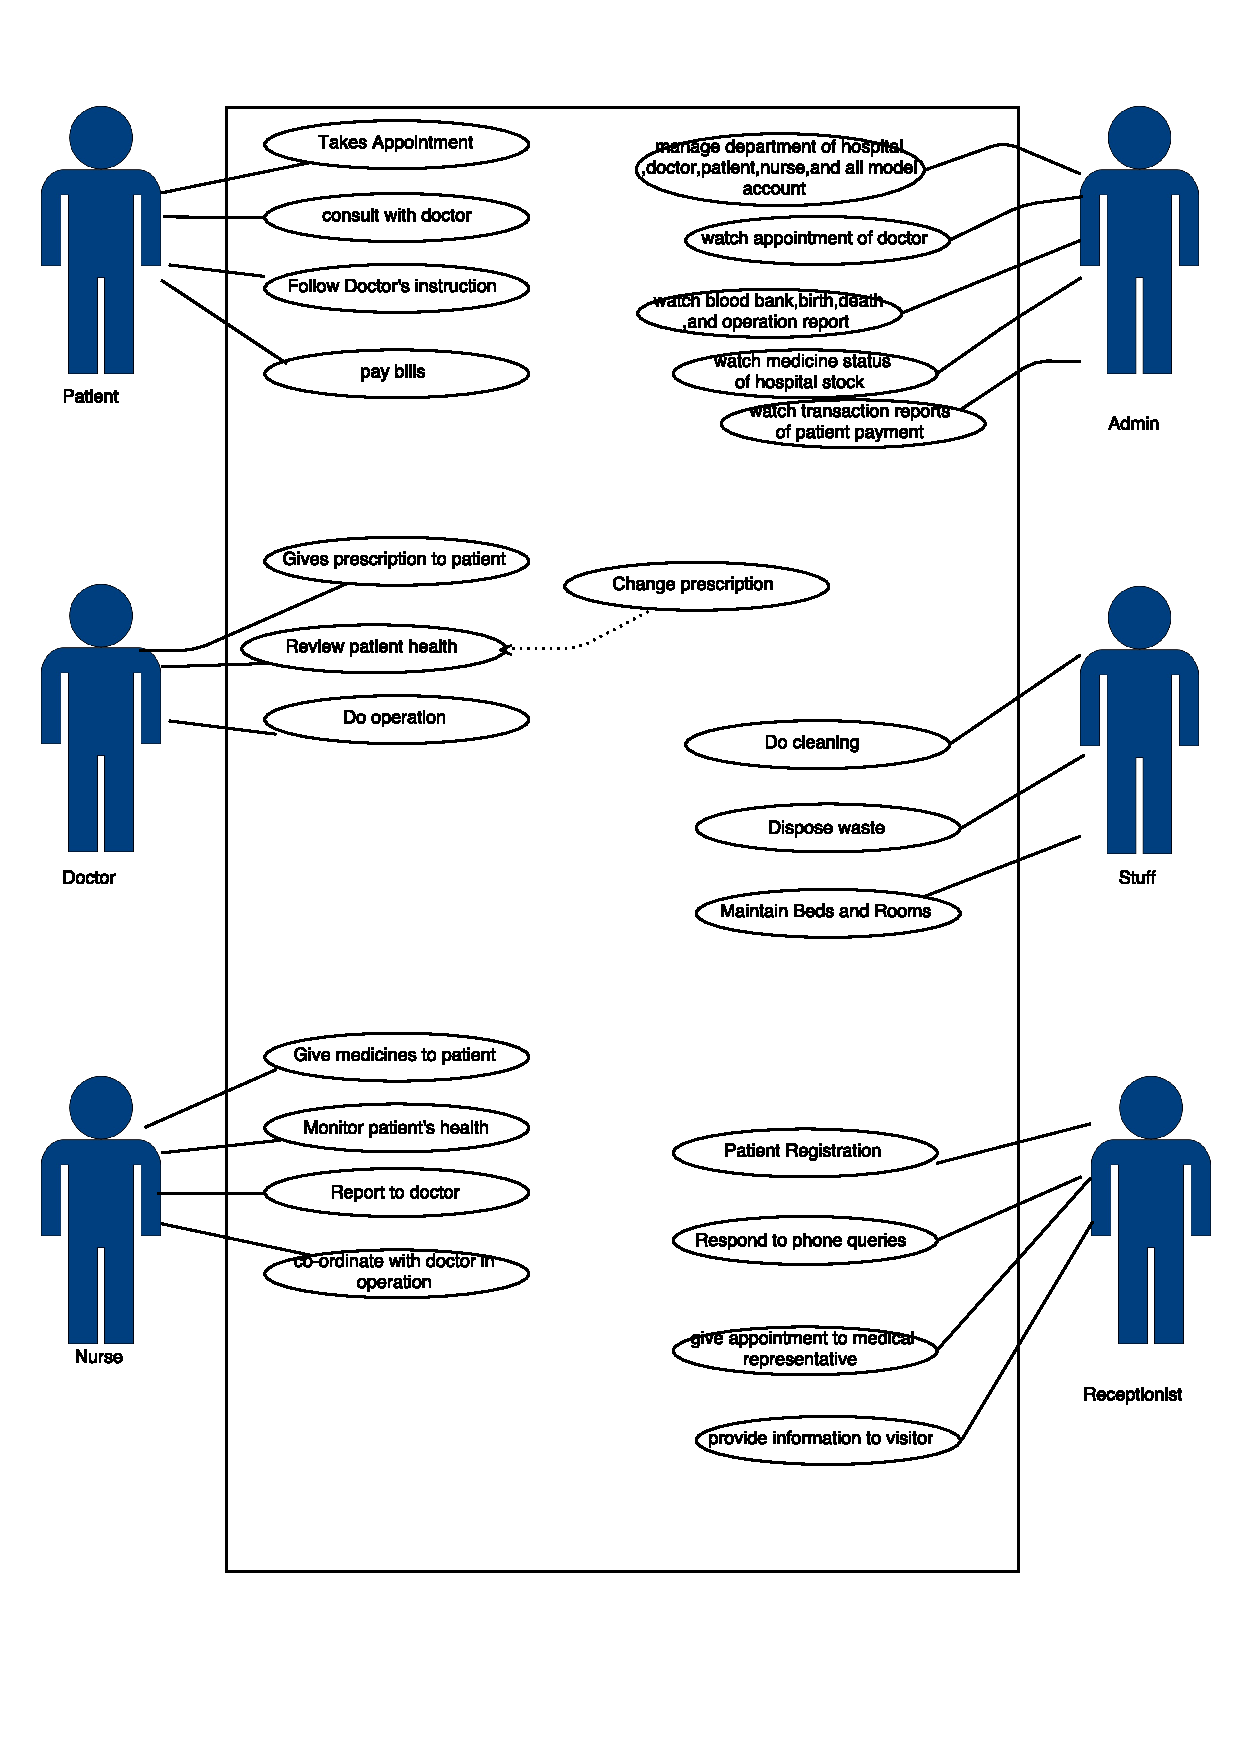
\includegraphics[width=15cm]{hospitalDiagram1.pdf}
\end{figure}
\newpage
\begin{figure}[h!]
\centering
  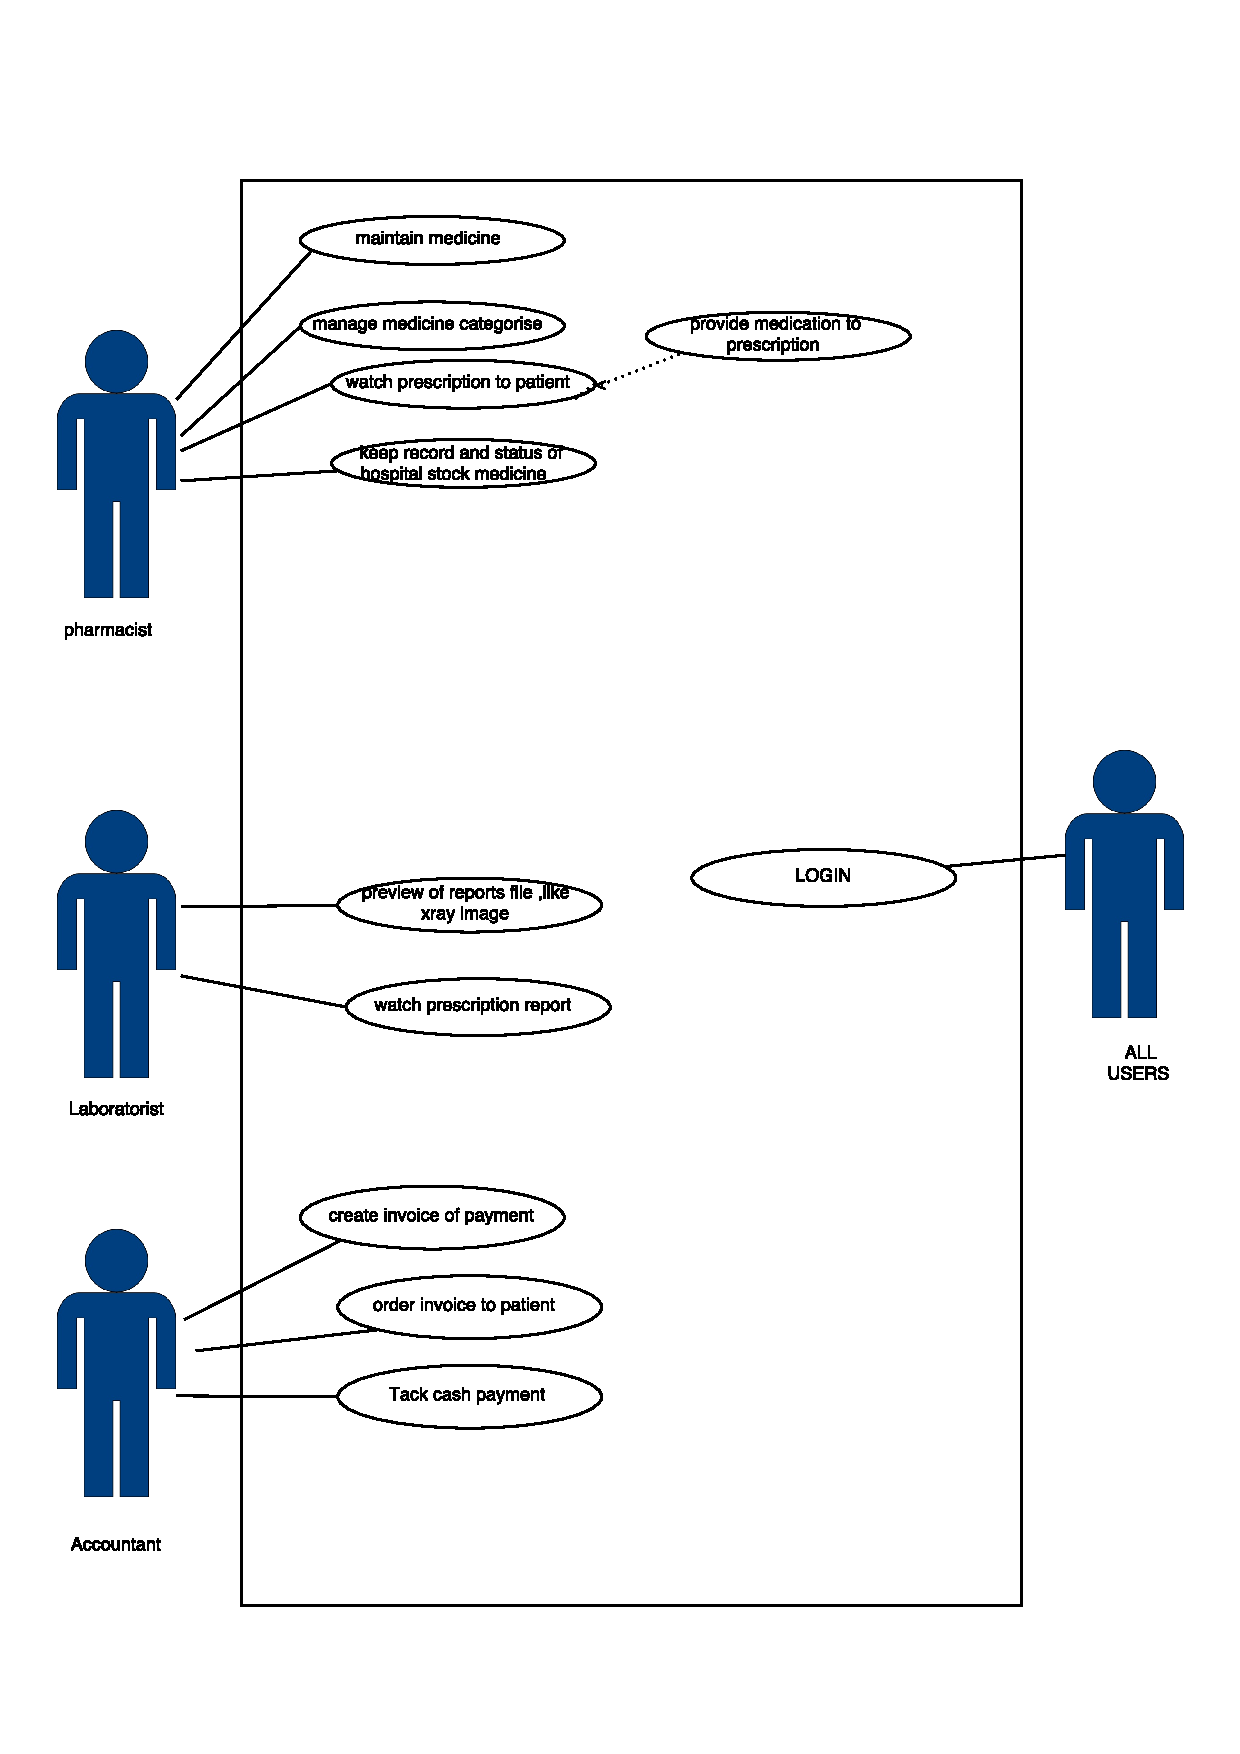
\includegraphics[width=15cm]{hospitalDiagram-2.pdf}
\end{figure}

\end{document}
